\documentclass[11pt,aspectratio=169]{beamer}

% Packages
% Shared content style for NN and NNDS. Written by Claude (2026-10-14).
%
% Everything that shared slides rely on lives here, loaded by both courses:
% colors, notation helpers and the card system. Course themes own only the
% presentation around the content (header, footer, title page, fonts, the
% \myalert color and where \SlideSource text goes). Change a definition here,
% never by redefining it in a course file, so the two courses cannot drift.

\usepackage{mathtools,amssymb,tcolorbox}
\tcbsetforeverylayer{autoparskip}

% Semantic colors
\definecolor{darkred}{rgb}{0.55,0,0}
\definecolor{darkpastelblue}{rgb}{0.47,0.62,0.8}
\definecolor{darkcerulean}{rgb}{0.03,0.27,0.49}
\definecolor{darkgreen}{rgb}{0,0.55,0}

% Figure palette (draw.io defaults)
\definecolor{titlecolor}{RGB}{245, 242, 238}
\definecolor{drawgray}{HTML}{666666}
\definecolor{drawgray_l}{HTML}{F5F5F5}
\definecolor{drawblue}{HTML}{6C8EBF}
\definecolor{drawblue_l}{HTML}{DAE8FC}
\definecolor{drawgreen}{HTML}{82B366}
\definecolor{drawgreen_l}{HTML}{D5E8D4}
\definecolor{draworange}{HTML}{D79B00}
\definecolor{draworange_l}{HTML}{FFE6CC}
\definecolor{drawyellow}{HTML}{D6B656}
\definecolor{drawyellow_l}{HTML}{FFF2CC}
\definecolor{drawred}{HTML}{B85450}
\definecolor{drawred_l}{HTML}{EA6B66}
\definecolor{drawviolet}{HTML}{9673A6}
\definecolor{drawviolet_l}{HTML}{E1D5E7}

% Notation
\newcommand{\vc}[1]{\boldsymbol{\mathbf{#1}}}
\DeclareMathOperator*{\argmax}{arg\,max}
\DeclareMathOperator*{\argmin}{arg\,min}

% Cards: blue for definitions and computable quantities, green for goals and
% stable formulations, orange for warnings and trade-offs, red for
% training-specific or problematic elements.
\tcbset{
	nndsblue/.style={colback=drawblue_l!35!white,colframe=drawblue,boxrule=0.8pt,arc=1mm},
	nndsgreen/.style={colback=drawgreen_l!35!white,colframe=drawgreen,boxrule=0.8pt,arc=1mm},
	nndsorange/.style={colback=draworange_l!35!white,colframe=draworange,boxrule=0.8pt,arc=1mm},
	nndsred/.style={colback=drawred_l!12!white,colframe=drawred,boxrule=0.8pt,arc=1mm}
}

% A card that opens with \[ would start with an empty paragraph line plus the
% display skip, leaving more room above than below (by an amount that differs
% between engines). Set that leading equation as a centered display-style line
% instead, so the space above it is the card padding, as below.
\makeatletter
\newcommand{\nndscardlead}{\futurelet\nndscard@next\nndscard@check}
% tcolorbox follows this hook with \ignorespaces; look past it.
\def\nndscard@check{\ifx\nndscard@next\ignorespaces
	\expandafter\nndscard@skip\else\expandafter\nndscard@test\fi}
\def\nndscard@skip\ignorespaces{\nndscard@test}
\newcommand{\nndscard@test}{\@ifnextchar\[{\nndscard@display}{}}
\def\nndscard@display\[#1\]{{\centering$\displaystyle#1$\par}\@ifnextchar\end{}{\vspace{\belowdisplayskip}}}
\makeatother

% Card text is ragged-right: narrow justified columns open wide word gaps,
% especially in NNDS, which never hyphenates. Fixed display spacing: when
% parallel cards share a height, stretchable skips would otherwise spread
% the content unevenly.
\tcbset{
	nndscard/.style={before upper={\raggedright
		\setlength{\abovedisplayskip}{6pt}\setlength{\belowdisplayskip}{6pt}%
		\setlength{\abovedisplayshortskip}{6pt}\setlength{\belowdisplayshortskip}{6pt}%
		\nndscardlead}},
	nndsblue/.append style={nndscard},
	nndsgreen/.append style={nndscard},
	nndsorange/.append style={nndscard},
	nndsred/.append style={nndscard}
}

% Parallel cards share a group name and get equal heights; the second argument
% (a fixed height used by older NNDS slides) is ignored.
\tcbset{courseheight/.style 2 args={equal height group=#1}}

\usepackage{tikz}

% Matrix shapes written under a symbol, e.g. \shape{\vc{Q}}{(T,D_k)}.
\usepackage{stackengine}
\stackMath
\def\sss{\scriptstyle \color{gray}}
\setstackgap{L}{12pt}
\def\stacktype{L}
\newcommand{\shape}[2]{\stackunder{#1}{\sss #2}}

% Transformer slides: colors and diagram styles (moved here from the NNDS
% transformers-settings.tex on 2026-11-16, when NN adopted the lecture).

% Query, key and value colors, reused in equations and figures.
\colorlet{qcolor}{drawviolet!80!black}
\colorlet{kcolor}{draworange!85!black}
\colorlet{vcolor}{darkcerulean}
\newcommand{\qc}[1]{{\color{qcolor}#1}}
\newcommand{\kc}[1]{{\color{kcolor}#1}}
\newcommand{\vcl}[1]{{\color{vcolor}#1}}

% Block-diagram styles, as in shared/slides/mlps.tex and the deeper-models deck.
\tikzset{
    nnblock/.style={
            draw=drawblue, fill=drawblue_l!25!white, rounded corners=2pt,
            minimum width=1.25cm, minimum height=0.65cm,
            inner sep=5pt, font=\small
        },
    nnother/.style={nnblock, draw=drawgreen, fill=drawgreen_l!25!white},
    nnmerge/.style={
            circle, draw=drawgray, fill=white,
            minimum size=0.55cm, inner sep=1pt, font=\small
        },
    nnedge/.style={->, thick, draw=drawgray}
}

% Full-size diagram styles for the transformer figures: arrows as in the
% attention figures (Stealth tips, gray), boxes at normal size.
\tikzset{
    tfarr/.style={-{Stealth[length=5pt]}, drawgray, line width=0.6pt},
    tfblk/.style={draw=drawblue, fill=drawblue_l!60, rounded corners=2pt,
            minimum height=0.75cm, minimum width=1.9cm, inner sep=4pt, font=\small},
    tfnorm/.style={tfblk, draw=drawgreen, fill=drawgreen_l!70},
    tfsum/.style={circle, draw=drawgray, fill=white, minimum size=0.45cm, inner sep=0pt, font=\small},
    tflab/.style={font=\scriptsize, text=black!60},
}

\usepackage{mathtools}
\usepackage{hyperref}
\usepackage{setspace}
\usepackage{tikz}
\usetikzlibrary{positioning}
\usepackage{ragged2e}
\usepackage{nicematrix}
\usepackage[compatibility=false]{caption}
\usepackage[framemethod=tikz]{mdframed}


% Theme
\usetheme{metropolis}
\metroset{subsectionpage=progressbar,sectionpage=none}
\setbeamertemplate{theorems}[numbered]

\usepackage{fontspec}
\defaultfontfeatures{LetterSpace=30}
\usepackage{microtype}

% Prefer flexible inter-word spacing over splitting words across lines.
\tolerance=1
\emergencystretch=\maxdimen
\hyphenpenalty=10000
\hbadness=10000


% Code
\usepackage{listings}
% Custom colors
\definecolor{codegreen}{rgb}{0,0.6,0}
\definecolor{codegray}{rgb}{0.5,0.5,0.5}
\definecolor{codepurple}{rgb}{0.58,0,0.82}
\definecolor{backcolour}{rgb}{0.95,0.95,0.92}
\definecolor{light-gray}{gray}{0.95}
% Python style for highlighting
\newcommand\pythonstyle{\lstset{
		backgroundcolor=\color{white},
		language=Python,
		basicstyle=\ttfamily\footnotesize,
		morekeywords={self},              % Add keywords here
		keywordstyle=\color{blue},
		stringstyle=\footnotesize\color{deepgreen},
		commentstyle=\color{codegreen},
		showstringspaces=false,
		frame=tb,
		numbers=left,
		numbersep=5pt,
		numberstyle=\tiny\color{gray},
		columns=fullflexible,
		numbersep=5pt,
		aboveskip=1em,
		showtabs=false,
		tabsize=2,
		gobble=3
	}}

% Python environment
\lstnewenvironment{python}[1][]
{
	\pythonstyle
	\lstset{#1}
}
{}
% Python for inline
\newcommand\pythoninline[1]{{\pythonstyle\lstinline!#1!}}

% Tables and justification
\newcommand{\ra}[1]{\renewcommand{\arraystretch}{#1}}
\justifying

% Subfigures
\setbeamertemplate{caption}[numbered]
\usepackage[caption=false,font=footnotesize]{subfig}

% Colors
\setbeamercolor{uppercolgreen}{fg=white,bg=green!35}
\setbeamercolor{lowercolgreen}{fg=black,bg=green!10}
\setbeamercolor{uppercolred}{fg=white,bg=red!35}
\setbeamercolor{lowercolred}{fg=black,bg=red!10}
\setbeamercolor{uppercolblue}{fg=white,bg=blue!35}
\setbeamercolor{lowercolblue}{fg=black,bg=blue!10}
\definecolor{deepblue}{rgb}{0,0,0.5}
\definecolor{deepred}{rgb}{0.6,0,0}
\definecolor{deepgreen}{rgb}{0,0.5,0}

% Mathematical commands
\newcommand{\pr}[1]{{#1\,}'}
\newcommand{\idx}[2]{{\color{darkpastelblue}[}#1{\color{darkpastelblue}]_{#2}}}
% Course switch for shared slides: \NNDSorNN{NNDS text}{NN text}.
\newcommand{\NNDSorNN}[2]{#1}

% Style commands
\newcommand{\myalert}[1]{{\color{darkred}\textbf{#1}}}

% White background on every slide, so figures with a white canvas blend in
% (Simone, 2026-10-14). whiteframe is kept as an alias for existing slides.
\setbeamercolor{background canvas}{bg=white}

% White frame (for images)
\newenvironment{whiteframe}[1]{
	\setbeamercolor{background canvas}{bg=white}
	\begin{frame}{#1}
		}{
	\end{frame}
}

\setbeamerfont{frametitle}{size=\normalsize}
\setbeamertemplate{frametitle}[default][right]
% Slimmer header, close to NN's share of the slide height (Simone, 2026-10-14).
\makeatletter
\patchcmd{\beamer@@tmpl@frametitle}{sep=0.3cm}{sep=0.2cm}{}{\PackageWarning{style}{frametitle padding not patched}}
\makeatother
{
}
%\setbeamercolor{frametitle}{fg=white,bg=black!75}

% No headline frame
\makeatletter
\newenvironment{noheadline}{
	\setbeamertemplate{headline}{}
	\addtobeamertemplate{frametitle}{\vspace*{-3.5\baselineskip}}{}
}{}
\makeatother

% Lists
\setbeamertemplate{itemize items}[triangle]

% Footnotes
\setbeamertemplate{footnote}%
{%
	\parindent 1.5em\noindent%
	\justifying\setstretch{0.7}%
	\hbox to 1em{\hfil\insertfootnotemark}\begin{scriptsize}\insertfootnotetext\end{scriptsize}\par%
}

% Footnote without number
\newcommand\blfootnote[1]{%
	\begingroup
	\renewcommand\thefootnote{}\footnote[frame]{\noindent#1}%
	\addtocounter{footnote}{-1}%
	\endgroup
}

% Slide sources: set in the frame footer beside the page number, so they
% take no room from the content. Zero height keeps the footline unchanged.
% Global, because the footline is typeset outside the frame's group; each
% frame starts empty.
\newcommand{\insertslidesource}{}
\newcommand{\SlideSource}[1]{\gdef\insertslidesource{#1}}
\AddToHook{env/frame/begin}{\gdef\insertslidesource{}}
\setbeamertemplate{frame footer}{%
	\ifx\insertslidesource\empty\else
		\smash{\parbox[b]{0.88\textwidth}{\raggedright\scriptsize\color{black!60}\insertslidesource}}%
	\fi}

% Theorems
\newcommand*{\theorembreak}{\usebeamertemplate{theorem end}\framebreak\usebeamertemplate{theorem begin}}
\newcounter{theo}[section]\setcounter{theo}{0}
\renewcommand{\thetheo}{\arabic{section}.\arabic{theo}}

\newenvironment{theo}[2][]{%
	\refstepcounter{theo}%
	\ifstrempty{#1}%
	{\mdfsetup{%
			frametitle={%
					\tikz[baseline=(current bounding box.east),outer sep=0pt]
					\node[anchor=east,rectangle,fill=red!10]
					{\strut Theorem~\thetheo};}}
	}%
	{\mdfsetup{%
			frametitle={%
					\tikz[baseline=(current bounding box.east),outer sep=0pt]
					\node[anchor=east,rectangle,fill=red!10]
					{\strut Theorem~\thetheo:~#1};}}%
	}%
	\mdfsetup{innertopmargin=5pt,linecolor=red!10,%
		linewidth=2pt,topline=true,%
		frametitleaboveskip=\dimexpr-\ht\strutbox\relax
	}
	\begin{mdframed}[]\relax%
		\label{#2}}{\end{mdframed}}

\usetikzlibrary{arrows.meta,calc}
\graphicspath{{assets/}{../../shared/assets/}}

\usepackage{annotate-equations}

% Written by Claude (2026-11-25): refresh of the NNDS 2024 Lecture 10
% (Recurrent models). Plan agreed with Simone on 2026-11-25 (vault: NNDS Slide
% Refresh Log): same order as 2024, shorter SSM part, new sections on modern
% linear recurrences and hybrid models at the end.

\begin{document}

{\usebackgroundtemplate{\tikz\node[opacity=0.4,inner sep=0]{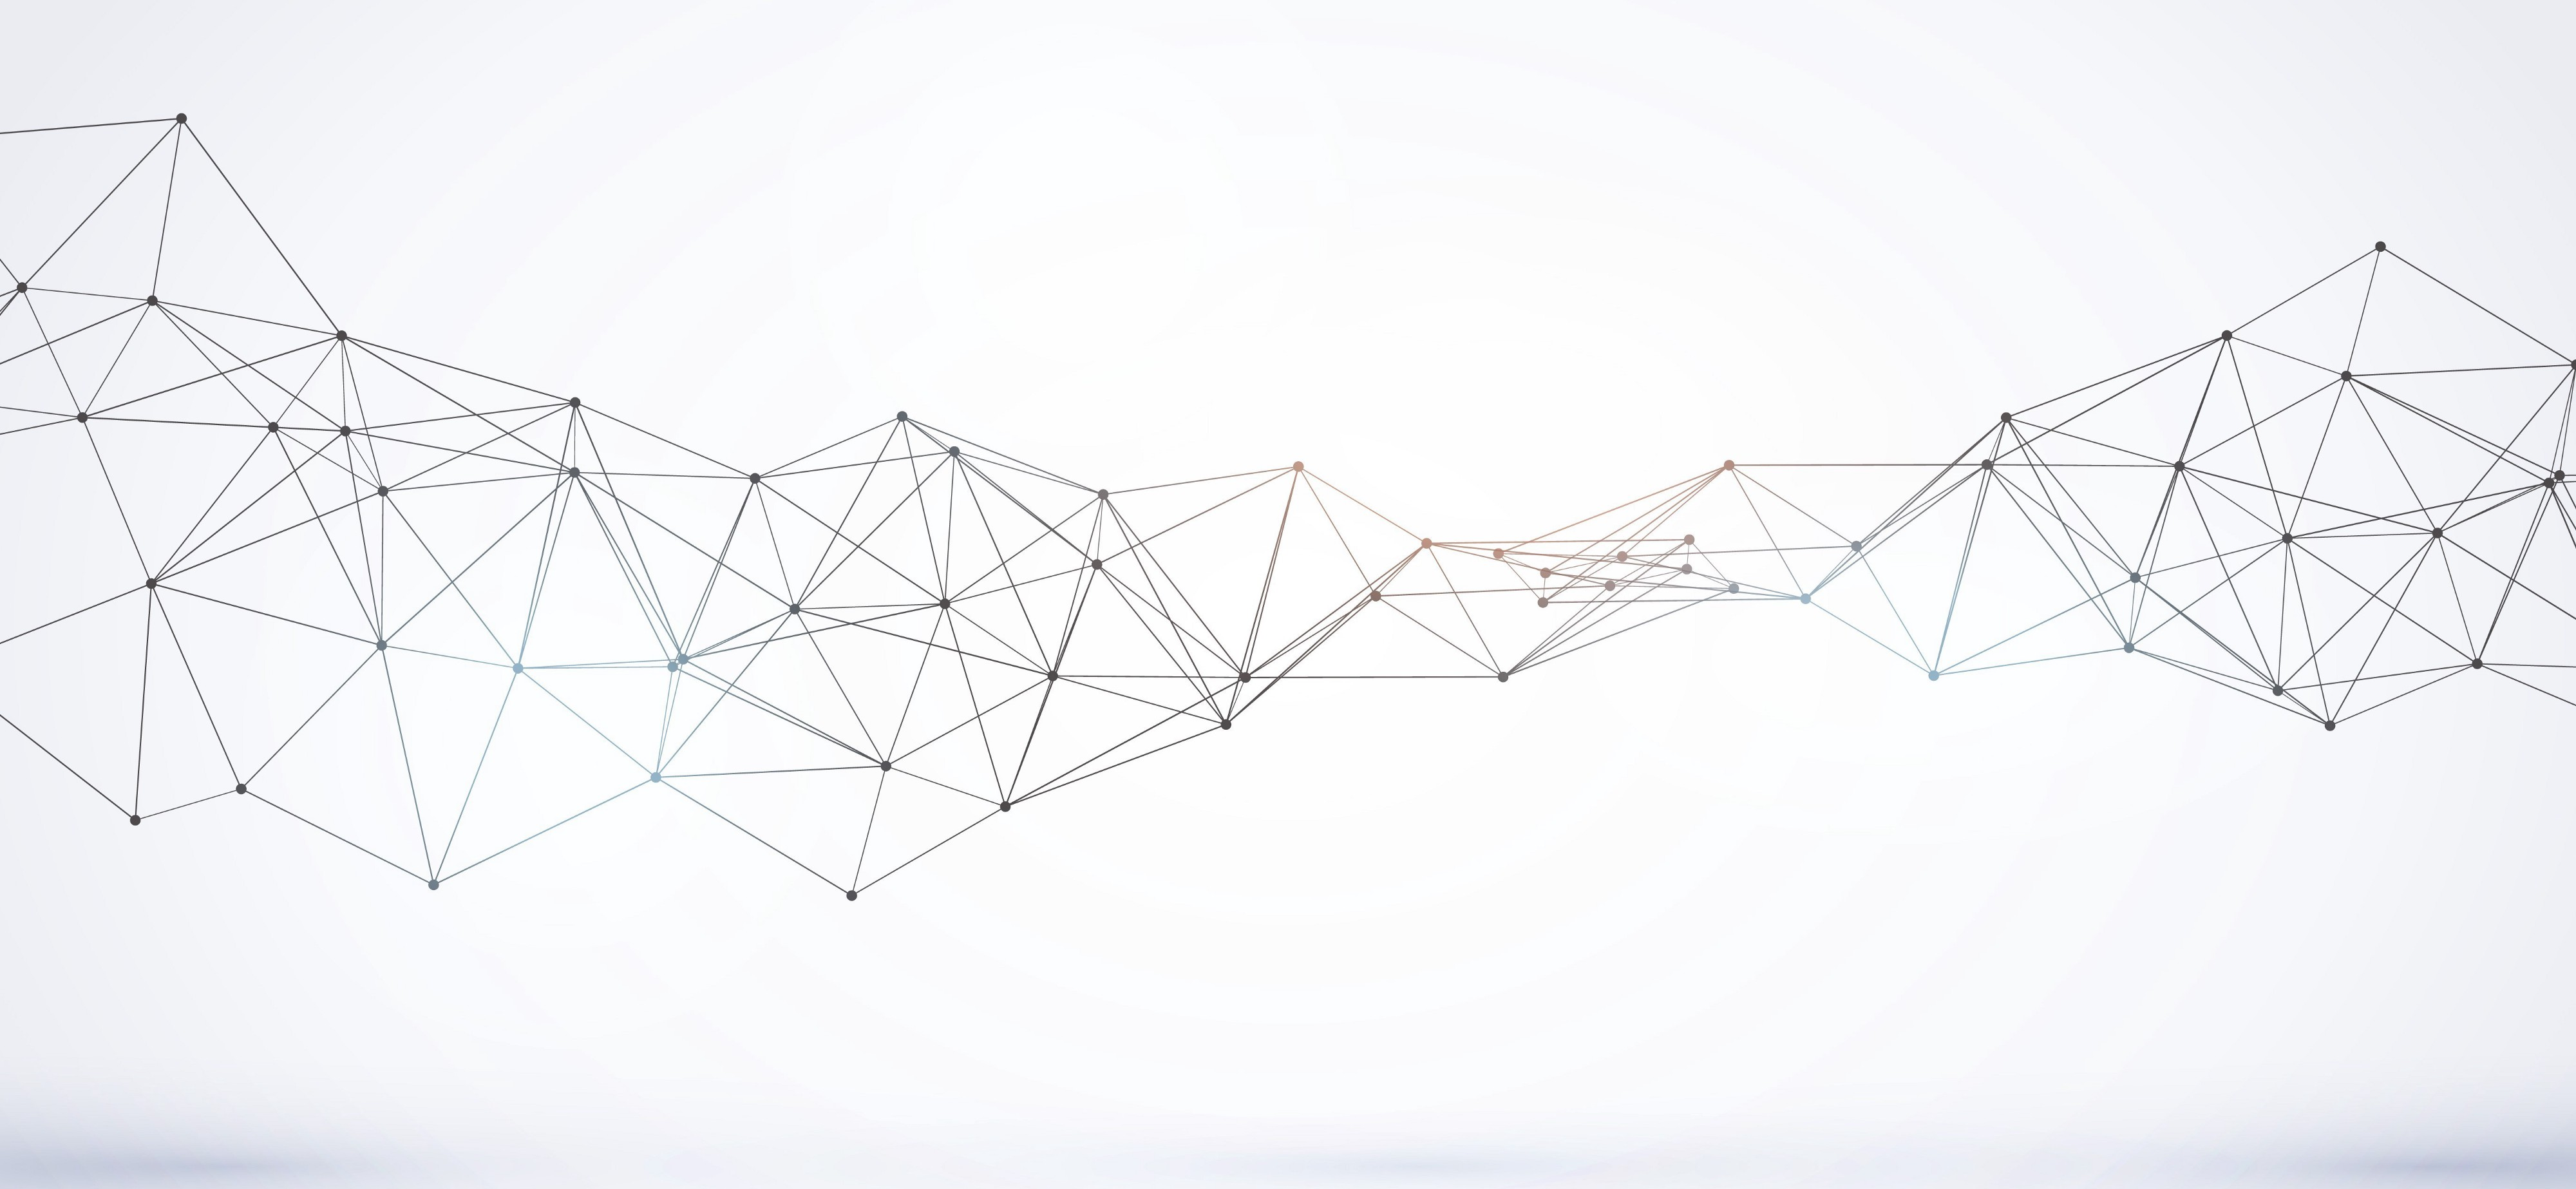
\includegraphics[width=\paperwidth,height=\paperheight]{images/header}};}%
\begin{frame}[plain]
    \vspace{0.5cm}
    \title{\large \begin{spacing}{1.0}Neural Networks for Data Science\end{spacing}\vspace{0.25em}
        \normalsize \begin{spacing}{1.0}\textbf{Master's Degree in Data Science}\end{spacing}\vspace{0.5em}}
    \subtitle{\Large \textbf{Recurrent models}}
    \date{
        {
\includegraphics[scale=0.8]{images/Uniroma1}}
    }
    \author{
        \setlength{\tabcolsep}{2pt}
        \begin{tabular}{rl}
            \textbf{Lecturer}: & S. Scardapane \\
        \end{tabular}
    }\titlepage
\end{frame}
}

\part{1}

\section{Linearized transformer}
\subsection{The model}

\begin{frame}{Convolutions, attention, and recurrence}
    \setlength{\parskip}{6pt}

    Up to now, we introduced two classes of models for dealing with sequences:
    \begin{enumerate}
        \setlength{\itemsep}{2pt}
        \item \myalert{Convolutional} models are parameter-efficient and have
              linear complexity in the sequence length $T$, but they are less
              efficient at handling \textit{long-range} dependencies.
        \item \myalert{Transformers} handle long-range dependencies, but their
              complexity is quadratic in $T$, and the KV cache grows linearly
              in $T$ (for Llama~3 8B, $17$\,GB for one sequence of $128$K
              tokens). Sliding windows bound the cache by dropping all but the
              last $w$ tokens.
    \end{enumerate}

    \begin{tcolorbox}[nndsgreen]
        A \textbf{\color{darkgreen}recurrent} layer keeps instead a
        \textbf{state} of fixed size, which summarizes all the tokens seen so
        far and is updated once per token, with constant memory and constant
        cost per step.
    \end{tcolorbox}

    \vspace{-2pt}
    \SlideSource{\href{https://arxiv.org/abs/2407.21783}{Grattafiori et al., Llama 3 (2024)}.}

\end{frame}

\begin{frame}{Linearized attention}
    \setlength{\parskip}{6pt}

    We begin with a generalization of the attention layer that can be written
    in a recurrent form. Consider again the SA layer with a generic
    scalar-valued attention function $\alpha(\cdot,\cdot)$ instead of the dot
    product:
    \[
        \vc{h}_t=\frac{\sum_{t'=1}^{T}\alpha\left(\qc{\vc{q}_t},\kc{\vc{k}_{t'}}\right)\vcl{\vc{v}_{t'}}}{\sum_{t'=1}^{T}\alpha\left(\qc{\vc{q}_t},\kc{\vc{k}_{t'}}\right)} \,,
    \]
    where for the standard SA, $\alpha(\vc{x},\vc{y})=\exp(\vc{x}^{\top}\vc{y}/\sqrt{D_k})$.

    \SlideSource{\href{https://arxiv.org/abs/2006.16236}{Katharopoulos et al., Transformers are RNNs: Fast autoregressive transformers with linear attention (2020)}, ICML.}

\end{frame}

\begin{frame}{Kernel functions}
    \setlength{\parskip}{6pt}

    Any non-negative $\alpha$ is a valid similarity function. In machine
    learning, these are known as \textbf{kernel functions}. Most kernel
    functions (e.g., polynomial, Gaussian) can be written as a generalized
    dot product
    \[
        \alpha(\vc{x},\vc{y})=\phi(\vc{x})^{\top}\phi(\vc{y})
    \]
    for some function $\phi:\mathbb{R}^{D_k}\rightarrow\mathbb{R}^{E}$
    performing a feature expansion. A \textbf{linearized attention} layer is
    obtained by using this $\alpha$ in the attention layer.

\end{frame}

\begin{frame}{Linearized attention layer}
    \setlength{\parskip}{6pt}

    Working out the calculation (see details in the book and in the paper; the
    key point is that $\phi(\qc{\vc{q}_t})$ does not depend on $t'$):
    \[
        \vc{h}_t=\frac{\phi(\qc{\vc{q}_t})^{\top}\sum_{t'=1}^{T}\phi(\kc{\vc{k}_{t'}})\vcl{\vc{v}_{t'}}^{\top}}{\phi(\qc{\vc{q}_t})^{\top}\sum_{t'=1}^{T}\phi(\kc{\vc{k}_{t'}})} \,.
    \]

    This is the \textbf{linearized attention} layer. The two sums do not
    depend on $t$, so we compute them once and reuse them for every token.
    Computing all outputs costs $\mathcal{O}(TED_v)$ instead of
    $\mathcal{O}(T^2D_k)$, which is linear in the sequence length and
    advantageous whenever $T$ is larger than $E$.

    However, the usefulness of the layer becomes apparent if we focus on a
    \textbf{causal} variant.

\end{frame}

\subsection{A recurrent formulation}

\begin{frame}{Causal variant}
    \setlength{\parskip}{6pt}

    A causal variant is obtained by masking all elements such that $t'>t$:

    \vspace{1.5em}
    \[
        \vc{h}_t=\frac{\phi(\qc{\vc{q}_t})^{\top}\eqnmarkbox[drawred]{mem}{\sum_{t'=1}^{\color{drawred}t}\phi(\kc{\vc{k}_{t'}})\vcl{\vc{v}_{t'}}^{\top}}}{\phi(\qc{\vc{q}_t})^{\top}\eqnmarkbox[drawgreen]{norm}{\sum_{t'=1}^{\color{drawred}t}\phi(\kc{\vc{k}_{t'}})}}
        =\frac{\phi(\qc{\vc{q}_t})^{\top}\vc{S}_t}{\phi(\qc{\vc{q}_t})^{\top}\vc{z}_t}
    \]
    \annotate[yshift=1em]{above,right}{mem}{Attention memory $\vc{S}_t\sim(E,D_v)$}
    \annotate[yshift=-1em]{below,right}{norm}{Normalizer memory $\vc{z}_t\sim(E)$}

\end{frame}

\begin{frame}{Recurrent formulation}
    \setlength{\parskip}{6pt}

    We can rewrite the two \textit{memories} recursively as:
    \begin{gather*}
        \vc{S}_t=\vc{S}_{t-1}+\phi(\kc{\vc{k}_t})\vcl{\vc{v}_t}^{\top} \\
        \vc{z}_t=\vc{z}_{t-1}+\phi(\kc{\vc{k}_t})
    \end{gather*}
    where the base case of the recurrence is given by their initialization:
    \[
        \vc{S}_0=\vc{0} \,, \qquad \vc{z}_0=\vc{0} \,.
    \]

    These equations, together with the readout of the previous slide, provide
    the complete \myalert{recurrent} variant of the layer.

\end{frame}

\begin{frame}{Properties of the layer}
    \setlength{\parskip}{6pt}

    \begin{itemize}
        \setlength{\itemsep}{5pt}
        \item Similarly to the implementation of batch normalization, this
              layer is \myalert{stateful}: $\vc{S}_t$ and $\vc{z}_t$ change for
              every token processed, and they are reinitialized at the end of
              the sequence.
        \item The update step has constant-time complexity, similarly to a
              convolutional layer, and the memory does not grow with $t$
              (unlike a KV cache).
        \item Can we implement this layer in parallel?
    \end{itemize}

    We call any layer of this form a \myalert{recurrent} layer.

\end{frame}

\begin{frame}[fragile]{Two ways of computing the layer}
    \setlength{\parskip}{5pt}

    With $\phi(x)=\operatorname{elu}(x)+1$ (Katharopoulos et al.), we can
    compute the causal layer as a masked attention without softmax, or with the
    two memories:

    \begin{python}[gobble=8,aboveskip=2pt,belowskip=2pt]
        q, k = F.elu(q) + 1, F.elu(k) + 1           # phi(q), phi(k): (T, E)
        A = torch.tril(q @ k.T)                     # parallel form: (T, T)
        h_par = (A @ v) / A.sum(-1, keepdim=True)
        S, z, h_rec = torch.zeros(E, Dv), torch.zeros(E), []
        for t in range(T):                          # recurrent form
            S = S + torch.outer(k[t], v[t]); z = z + k[t]
            h_rec.append(q[t] @ S / (q[t] @ z))
        torch.allclose(h_par, torch.stack(h_rec), atol=1e-5)   # True
    \end{python}

    The parallel form costs $\mathcal{O}(T^2)$ like attention, while the
    recurrent form is linear in $T$ but runs one token at a time. We will see
    how to get the best of both.

\end{frame}

\section{Recurrent layers}
\subsection{General formulation}

\begin{frame}{General properties}
    \setlength{\parskip}{6pt}

    To provide a general definition, let us abstract away some key properties:

    \begin{enumerate}
        \setlength{\itemsep}{5pt}
        \item First, we need a fixed-size \textbf{state} which encodes all
              useful information up to the current element in the sequence. We
              denote it generically as $\vc{s}_t$, and from now on we assume it
              is a vector.
        \item Second, we need a \textbf{transition function} (recurrence) that
              updates the state vector based on the previous value and the
              value of the current token, which we denote as
              $f(\vc{s}_{t-1},\vc{x}_t)$.
        \item Third, we need a \textbf{readout function} to compute the output
              for the $t$-th element of the sequence. We denote it as
              $g(\vc{s}_t,\vc{x}_t)$.
    \end{enumerate}

\end{frame}

\begin{whiteframe}{Recurrent layers}

    \begin{figure}
        \centering
        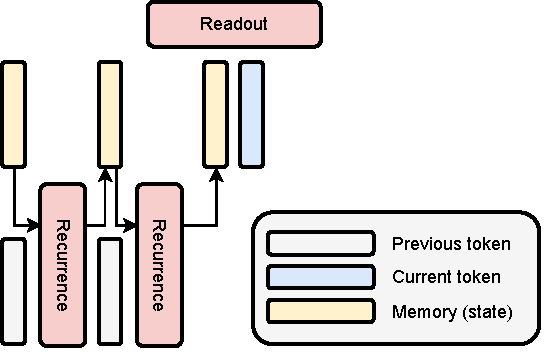
\includegraphics[width=0.6\columnwidth]{images/recurrent/recurrence.pdf}
        \caption{Overview of a recurrent layer: past tokens are shown in gray,
            current input token in blue, the memory state in yellow.}
    \end{figure}

\end{whiteframe}

\begin{frame}{General formulation}
    \setlength{\parskip}{6pt}

    Based on the previous definition, given a sequence of tokens
    $\vc{x}_1,\vc{x}_2,\ldots$, a recurrent layer can be written as:
    \begin{gather*}
        \vc{s}_t=f(\vc{s}_{t-1},\vc{x}_t) \\
        \vc{h}_t=g(\vc{s}_t,\vc{x}_t)
    \end{gather*}
    where $\vc{s}_0=\vc{0}$. The size of the state vector,
    $\vc{s}_t\sim(E)$, and the size of the output vector,
    $\vc{h}_t\sim(O)$, are hyper-parameters. We call $f$ the
    \textbf{state transition} function and $g$ the \textbf{readout} function.

    \myalert{Recurrent neural networks} (RNNs) are built by stacking multiple
    layers of this form.

\end{frame}

\begin{frame}{Additional comments}
    \setlength{\parskip}{6pt}

    \begin{itemize}
        \setlength{\itemsep}{4pt}
        \item RNNs are fundamentally input-driven dynamical systems.
        \item They are causal layers by definition.
        \item In control engineering, they are known as
              \myalert{state-space models}.
    \end{itemize}

    For tasks in which causality is unnecessary, \textbf{bidirectional
    layers} can be defined. In a bidirectional layer we initialize two
    recurrent layers (with separate parameters), one of which processes the
    sequence left-to-right, and the second one right-to-left. Their output
    states are then concatenated to provide the final output.

\end{frame}

\subsection{Vanilla recurrent layers}

\begin{frame}{Basic recurrent layer}
    \setlength{\parskip}{6pt}

    Historically, recurrent layers were instantiated by considering two
    fully-connected layers as transition and readout functions:
    \begin{gather*}
        f(\vc{s}_{t-1},\vc{x}_t)=\phi(\vc{A}\vc{s}_{t-1}+\vc{B}\vc{x}_t) \\
        g(\vc{s}_t,\vc{x}_t)=\vc{C}\vc{s}_t+\vc{D}\vc{x}_t
    \end{gather*}

    The layer has four trainable matrices $\vc{A}\sim(E,E)$,
    $\vc{B}\sim(E,D)$, $\vc{C}\sim(O,E)$, and $\vc{D}\sim(O,D)$, where $D$ is
    the input dimensionality (the size of each token). This is known generally
    as \textit{the} recurrent layer, or vanilla recurrent layer, or Elman
    recurrent network.

\end{frame}

\begin{frame}[fragile]{The recurrent layer in code}
    \setlength{\parskip}{5pt}

    \begin{python}[gobble=8,aboveskip=2pt,belowskip=2pt]
        class RNN(nn.Module):
            def __init__(self, D, E, O):
                super().__init__()
                self.A, self.B = nn.Linear(E, E, bias=False), nn.Linear(D, E)
                self.C, self.D = nn.Linear(E, O), nn.Linear(D, O, bias=False)
            def forward(self, x):                          # x: (B, T, D)
                s = x.new_zeros(x.shape[0], self.A.in_features)    # s_0 = 0, (B, E)
                h = []
                for t in range(x.shape[1]):                # one step per token
                    s = torch.tanh(self.A(s) + self.B(x[:, t]))
                    h.append(self.C(s) + self.D(x[:, t]))
                return torch.stack(h, dim=1)               # (B, T, O)
    \end{python}

    We can vectorize over the batch, but not over $t$. PyTorch's
    \pythoninline{nn.RNN} implements the same transition and returns the
    states $\vc{s}_t$.

\end{frame}

\begin{frame}{Issues}
    \setlength{\parskip}{6pt}

    This family of recurrent layers has multiple issues, e.g.:

    \begin{itemize}
        \setlength{\itemsep}{5pt}
        \item The computation cannot be parallelized and it must be executed
              with a for-loop operation. Even on recent GPUs with customized
              kernels, this is computationally expensive compared to other
              types of layers.
        \item The gradient computation requires to back-propagate through all
              transition functions (\textbf{backpropagation through time},
              BPTT), which might create instabilities due to the non-linearity
              (see the full computation in the book).
    \end{itemize}

    For these reasons, they fell out of favour compared to alternative
    attention-based models.

\end{frame}

\begin{whiteframe}{Backpropagation through time}

    \begin{figure}
        \centering
        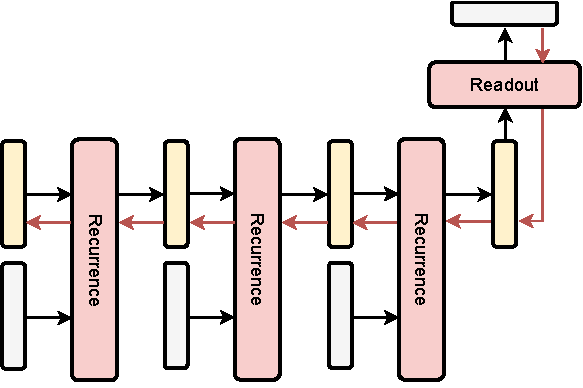
\includegraphics[height=0.62\textheight]{images/recurrent/recurrence_backward.pdf}
        \caption{Backward pass for a recurrent layer: the adjoint values have
            to be propagated through all the transition steps. Each state then
            contributes a single term to the full gradient of the parameters.}
    \end{figure}

\end{whiteframe}

\subsection{Gated recurrent layers}

\begin{frame}{Gated recurrent layers}
    \setlength{\parskip}{6pt}

    One issue of RNNs is that the entire state gets overwritten at each
    transition. However, for many sequences, only a few elements of these
    transitions are important and we may prefer to sparsify the transition
    step. This can be controlled by the introduction of so-called
    \textbf{gate} elements.

    We consider the simplest form of gated RNN, called \textbf{light gated
    recurrent unit} (Li-GRU), having a single gate.

    \SlideSource{\href{https://arxiv.org/abs/1803.10225}{Ravanelli et al., Light gated recurrent units for speech recognition (2018)}, IEEE TETCI.}

\end{frame}

\begin{frame}{What is a gate?}
    \setlength{\parskip}{6pt}

    A gating function is a layer that outputs values in the range $[0,1]$
    that can be used to ``mask'' the input. As an example, a gate over the
    state can be obtained by a fully-connected layer with a sigmoid activation
    function:
    \[
        \gamma(\vc{s}_{t-1},\vc{x}_t)=\sigma\left(\vc{V}\vc{s}_{t-1}+\vc{U}\vc{x}_t\right)
    \]

    If $\gamma_i\approx 0$, the $i$-th feature of the state should be kept
    untouched, while if $\gamma_i\approx 1$, we should propagate its updated
    value as output.

\end{frame}

\begin{frame}{The Li-GRU model}
    \setlength{\parskip}{6pt}

    We can obtain a gated layer by combining a gate with the transition
    function:
    \begin{align*}
        f(\vc{s}_{t-1},\vc{x}_t)= & \overbrace{\gamma(\vc{s}_{t-1},\vc{x}_t)\odot\left(\vc{A}\vc{s}_{t-1}+\vc{B}\vc{x}_t\right)}^{\text{New values}} \\
                                  & +\underbrace{(1-\gamma(\vc{s}_{t-1},\vc{x}_t))\odot\vc{s}_{t-1}}_{\text{Old values}}
    \end{align*}

    This can be seen as a soft (differentiable) approximation to a ``real''
    gate having only binary values, or as a convex combination of the original
    layer and a skip connection.

\end{frame}

\begin{frame}{Other gated models}
    \setlength{\parskip}{6pt}

    Other famous models in this category include the \textbf{gated recurrent
    unit} (GRU) with two gates and the \textbf{long short-term memory} (LSTM)
    network with three gates.

    LSTMs were the first gated variant to be introduced in the literature, and
    for a long time they have been the most successful deep architecture for
    processing sequences. Research on LSTM models is still very active.

    \SlideSource{\href{https://arxiv.org/abs/2405.04517}{Beck et al., xLSTM: Extended Long Short-Term Memory (2024)}, NeurIPS.}

\end{frame}

\section{Structured SSMs}
\subsection{A linear transition function}

\begin{frame}{Structured SSMs}
    \setlength{\parskip}{6pt}

    Suppose we remove the nonlinearity in the transition function:
    \begin{gather*}
        f(\vc{s}_{t-1},\vc{x}_t)=\vc{A}\vc{s}_{t-1}+\vc{B}\vc{x}_t \\
        g(\vc{s}_t,\vc{x}_t)=\vc{C}\vc{s}_t+\vc{D}\vc{x}_t
    \end{gather*}

    We call this a \textbf{state space model} (improperly, as every RNN is an
    SSM) or better a \textit{structured} SSM, as we will see that the
    transition matrix needs to be properly constrained to make this work. An
    SSM layer is ``less expressive'' than a vanilla layer, but this can be
    recovered by adding activation functions after the output, or by
    interleaving these layers with token-wise MLPs.

    \SlideSource{\href{https://arxiv.org/abs/2307.11888}{Orvieto et al., On the universality of linear recurrences followed by nonlinear projections (2023)}.}

\end{frame}

\begin{frame}{An historical note}
    \setlength{\parskip}{6pt}

    Interest in structured SSMs started in 2020 with HiPPO
    (\textbf{High-Order Polynomial Projection Operator}), a construction of
    $\vc{A}$ that compresses a one-dimensional input sequence according to a
    pre-defined reconstruction criterion. Stacks of SSM layers based on HiPPO
    followed: the \textbf{S4} layer in 2021 and the simplified S5 layer in
    2022.

    We focus on a simplified variant known as the \textbf{linear recurrent
    unit} (LRU).

    \SlideSource{\href{https://arxiv.org/abs/2008.07669}{Gu et al., HiPPO (2020)}, NeurIPS; \href{https://arxiv.org/abs/2111.00396}{Gu et al., S4 (2022)}, ICLR; \href{https://arxiv.org/abs/2303.06349}{Orvieto et al., Resurrecting recurrent neural networks for long sequences (2023)}, ICML.}

\end{frame}

\begin{frame}{Convolutional view}
    \setlength{\parskip}{6pt}

    Because of linearity, the recurrence has a closed-form solution:
    \[
        \vc{s}_t=\sum_{t'=1}^{t}\vc{A}^{t-t'}\vc{B}\vc{x}_{t'} \,.
    \]

    We can exploit this equation in two ways: as a convolution, or as a
    parallel scan. Stacking all coefficients into a rank-3 tensor $K$, all
    states are a single 1D convolution between
    $\vc{X}\sim(T,D)$ and a filter as long as the sequence (a \textit{long}
    convolution):
    \[
        K=\operatorname{stack}\left(\vc{A}^{T-1}\vc{B},\ldots,\vc{A}\vc{B},\vc{B}\right) \,, \qquad
        \vc{S}=\operatorname{Conv1D}(\vc{X},K) \,.
    \]
    The original structured SSMs computed it in the frequency domain, where a
    convolution becomes a multiplication.

    \SlideSource{\href{https://arxiv.org/abs/2110.13985}{Gu et al., Linear state space layers (2021)}, NeurIPS.}

\end{frame}

\subsection{Associative scans}

\begin{frame}{An interlude: associative scans}
    \setlength{\parskip}{6pt}

    \begin{columns}[c,onlytextwidth]
        \begin{column}{0.52\textwidth}
            \setlength{\parskip}{6pt}
            Consider a sequence of elements $(x_1,x_2,\ldots,x_n)$, and a
            binary associative operation $\star$. We want to compute all
            partial applications:
            \[
                {\color{drawred}x_1}, \;\; {\color{drawgreen}x_1\star x_2}, \;\; {\color{drawblue}x_1\star x_2\star x_3}, \;\; \ldots
            \]
            An iterative algorithm adds one element at every iteration.
            Exploiting associativity, we can instead compute multiple pairs
            of elements in parallel and then aggregate them recursively.
        \end{column}
        \begin{column}{0.44\textwidth}
            \begin{figure}
                \centering
                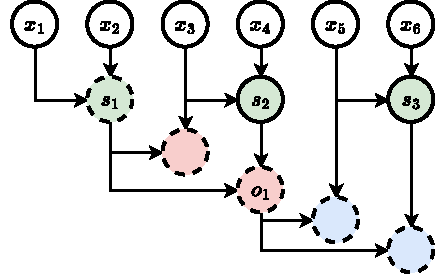
\includegraphics[width=0.9\textwidth]{images/recurrent/associative_scan.pdf}
                \caption{\scriptsize Parallel scan on six elements: circles of
                    the same color can be computed in parallel; dashed circles
                    are the outputs.}
            \end{figure}
        \end{column}
    \end{columns}

\end{frame}

\begin{frame}{A worked-out example}
    \setlength{\parskip}{6pt}

    Consider six elements $x_1,\ldots,x_6$, and denote by $\hat{x}_i$ the
    $i$-th prefix we want to compute (arrows denote outputs of the algorithm):

    \begin{columns}[T,onlytextwidth]
        \begin{column}{0.32\textwidth}
            \centering\textbf{Level 1}
            \begin{align*}
                s_1=x_1\star x_2 & \rightarrow\hat{x}_2 \\
                s_2=x_3\star x_4 &                      \\
                s_3=x_5\star x_6 &
            \end{align*}
        \end{column}
        \begin{column}{0.32\textwidth}
            \centering\textbf{Level 2}
            \begin{align*}
                s_1\star x_3     & \rightarrow\hat{x}_3 \\
                o_1=s_1\star s_2 & \rightarrow\hat{x}_4
            \end{align*}
        \end{column}
        \begin{column}{0.32\textwidth}
            \centering\textbf{Level 3}
            \begin{align*}
                o_1\star x_5 & \rightarrow\hat{x}_5 \\
                o_1\star s_3 & \rightarrow\hat{x}_6
            \end{align*}
        \end{column}
    \end{columns}

    \medskip
    We made $7$ applications of $\star$ instead of $5$, but the operations
    inside each level are independent, so with $3$ threads we need only $3$
    sequential steps. In general, a balanced scheme needs
    $\mathcal{O}(\log n)$ sequential steps and $\mathcal{O}(n)$ applications
    of $\star$ in total. An example of implementation is the
    \href{https://jax.readthedocs.io/en/latest/_autosummary/jax.lax.associative_scan.html}{associative scan function in JAX}.

    \SlideSource{\href{https://www.cs.cmu.edu/~guyb/papers/Ble93.pdf}{Blelloch, Prefix sums and their applications (1990)}.}

\end{frame}

\begin{frame}{SSMs and parallel scans}
    \setlength{\parskip}{6pt}

    The transition function in a linear SSM is an example of an all-prefix-sums
    problem. We define the elements of our sequence as pairs
    $x_t=(\vc{A},\vc{B}\vc{x}_t)$, and the binary operator as:
    \[
        (\vc{Z},\vc{z})\star(\vc{V},\vc{v})=(\vc{V}\vc{Z},\vc{V}\vc{z}+\vc{v}) \,.
    \]
    The prefixes of $\star$ are then given by:
    \[
        x_1\star x_2\star\ldots\star x_t=(\vc{A}^t,\vc{s}_t) \,.
    \]

    A parallel scan gives us the powers of $\vc{A}$ and all the states of the
    layer. However, each application of $\star$
    multiplies two $(E,E)$ matrices, which costs $\mathcal{O}(E^3)$. To make
    the entire procedure viable, we need to constrain $\vc{A}$ so that its
    powers can be computed more efficiently.

    \SlideSource{\href{https://arxiv.org/abs/2208.04933}{Smith et al., Simplified state space layers for sequence modeling (2023)}, ICLR.}

\end{frame}

\subsection{Diagonal SSMs}

\begin{frame}{Diagonal SSMs}
    \setlength{\parskip}{5pt}

    A common strategy is to work with diagonal transition matrices, whose
    powers are the powers of the diagonal entries. A square matrix $\vc{A}$ is
    \textbf{diagonalizable} if we can find an invertible matrix $\vc{P}$ and
    a diagonal matrix $\Lambda$ such that:
    \[
        \vc{A}=\vc{P}\Lambda\vc{P}^{-1} \,, \qquad \text{hence} \qquad
        \vc{A}^t=\vc{P}\Lambda^t\vc{P}^{-1} \,.
    \]
    If the transition matrix is diagonalizable, we substitute this in the
    closed form and multiply on both sides by $\vc{P}^{-1}$:

    \vspace{1.2em}
    \[
        \eqnmarkbox[drawred]{ns}{\vc{P}^{-1}\vc{s}_t}=\sum_{t'=1}^{t}\Lambda^{t-t'}\eqnmarkbox[drawgreen]{nb}{\vc{P}^{-1}\vc{B}}\vc{x}_{t'}
        \qquad\qquad
        \vc{h}_t=\eqnmarkbox[drawblue]{nc}{\vc{C}\vc{P}}\vc{P}^{-1}\vc{s}_t+\vc{D}\vc{x}_t
    \]
    \annotate[yshift=-0.6em]{below,left}{ns}{New state vector $\bar{\vc{s}}_t$}
    \annotate[yshift=-0.6em]{below,right}{nb}{New input-state matrix $\bar{\vc{B}}$}
    \annotate[yshift=0.6em]{above,right}{nc}{New readout matrix $\bar{\vc{C}}$}

\end{frame}

\begin{frame}{Diagonal SSMs (2)}
    \setlength{\parskip}{6pt}

    Putting everything together:
    \begin{gather*}
        \bar{\vc{s}}_t=\Lambda\bar{\vc{s}}_{t-1}+\bar{\vc{B}}\vc{x}_t \\
        \vc{h}_t=\bar{\vc{C}}\bar{\vc{s}}_t+\vc{D}\vc{x}_t
    \end{gather*}
    Hence, we can directly train $\Lambda=\operatorname{diag}(\vc{\lambda})$
    with $\vc{\lambda}\sim(E)$, $\bar{\vc{B}}\sim(E,D)$,
    $\bar{\vc{C}}\sim(O,E)$ and $\vc{D}\sim(O,D)$. In the parallel scan, the
    product of two $(E,E)$ matrices becomes an elementwise product of two
    vectors, which costs $\mathcal{O}(E)$.

    Not all matrices can be diagonalized, but an approximate diagonalization
    always exists if we allow complex-valued entries in $\vc{P}$ and
    $\Lambda$. We also need $|\lambda_i|<1$ to avoid diverging dynamics, which
    the LRU guarantees with the parameterization
    $\lambda_i=\exp(-\exp(\nu_i)+\mathrm{i}\,\theta_i)$.

    \SlideSource{\href{https://arxiv.org/abs/2303.06349}{Orvieto et al., Resurrecting recurrent neural networks for long sequences (2023)}, ICML.}

\end{frame}

\subsection{Selective SSMs}

\begin{frame}{Linear attention layers are SSMs}
    \setlength{\parskip}{6pt}

    Despite their differences, all the models we saw are connected. For
    example, consider a linearized attention layer where we ignore the
    denominator:
    \begin{gather*}
        \vc{S}_t=\vc{S}_{t-1}+\phi(\kc{\vc{k}_t})\vcl{\vc{v}_t}^{\top} \\
        \vc{h}_t=\phi(\qc{\vc{q}_t})^{\top}\vc{S}_t
    \end{gather*}

    This has the form of an SSM layer, except that some matrices (e.g.,
    $\vc{C}=\phi(\qc{\vc{q}_t})^{\top}$) are not fixed, but they depend on the
    specific input token. This has inspired another class of SSM layers whose
    matrices are not constrained to be time-invariant, which have been called
    \textbf{selective} SSMs.

\end{frame}

\begin{frame}{The Mamba block}
    \setlength{\parskip}{6pt}

    We consider the Mamba layer, which introduced the idea of selective SSMs.
    The core idea is to make some of the matrices of the SSM token-dependent:
    \begin{gather*}
        \vc{s}_t=A(\vc{x}_t)\vc{s}_{t-1}+B(\vc{x}_t)\vc{x}_t \\
        \vc{h}_t=C(\vc{x}_t)\vc{s}_t+\vc{D}\vc{x}_t
    \end{gather*}
    where $B(\bullet)$ and $C(\bullet)$ are linear projections of their input
    tokens, and $A(\bullet)$ is diagonal with entries in $(0,1)$, computed
    from a learned decay and a token-dependent step size. To make this
    feasible, the layer is applied to each channel of the input independently,
    so that all matrices of the SSM can be represented with a single vector of
    values.

    \SlideSource{\href{https://arxiv.org/abs/2312.00752}{Gu and Dao, Mamba: Linear-time sequence modeling with selective state spaces (2024)}, COLM.}

\end{frame}

\begin{frame}{Additional considerations}
    \setlength{\parskip}{6pt}

    Because the matrices change with every token, the layer loses the
    convolutional view (there is no fixed filter $K$). The parallel scan still
    works, since $\star$ only needs a different diagonal $A(\vc{x}_t)$ at every
    step, but the states are large ($E$ values for each of the $D$ channels).
    Mamba uses a hardware-aware scan which keeps them in the fast memory of
    the GPU instead of writing all of them to main memory.

    To make the overall architecture simpler, Mamba avoids alternating MLPs
    and SSMs, in favour of a gated architecture where an MLP is used to weight
    the outputs from the SSM. It also combines the model with the idea of
    multiple projections from transformers, and an additional depthwise
    convolution is added for improved flexibility.

\end{frame}

\begin{whiteframe}{Visualization of the Mamba layer}

    \begin{figure}
        \centering
        \hspace{2em}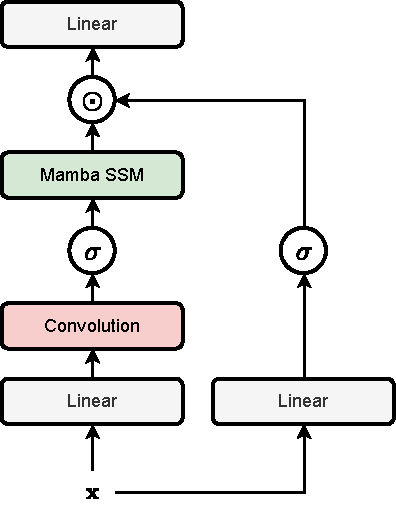
\includegraphics[height=0.68\textheight]{images/recurrent/mamba.pdf}
        \caption{Mamba block (residual connections around the block and
            normalization are not shown). $\sigma$ is the sigmoid function.}
    \end{figure}

\end{whiteframe}

\begin{frame}{Further readings}
    \setlength{\parskip}{6pt}

    \begin{itemize}
        \item \textbf{Chapter 13} of the book.
    \end{itemize}

\end{frame}

\end{document}
